% \RequirePackage{lineno}
\documentclass[twocolumn,preprintnumbers,amsmath,amssymb,superscriptaddress]{revtex4}
%\usepackage[pdftex]{graphicx}

\usepackage{amsmath,amsfonts,amssymb}
\usepackage[english]{babel}
\usepackage[latin1]{inputenc}
\usepackage[T1]{fontenc}
\usepackage{color}
\usepackage{float}
\usepackage{verbatim}
\usepackage{graphicx}
\usepackage{bm}
\usepackage{mathtools}
\usepackage{stmaryrd}
\usepackage{anyfontsize}


%\usepackage{epstopdf}
%\usepackage{array}
%\usepackage{tabularx}
%\usepackage{multirow}
\usepackage{color}
%\usepackage{multibox}
%\usepackage{rotating}
\usepackage{lineno}
%\usepackage[left]{lineno}
\usepackage[comma,sort&compress]{natbib}
\bibpunct{}{}{,}{s}{}{;}
%\usepackage{authblk}
%\usepackage{multicol}

\bibliographystyle{naturemag}

% \usepackage{bibunits}

% \linenumbers
% \setlength\linenumbersep{3pt}

\begin{document}


\author{Justin D. Yeakel,${}^{1,2,*}$, Christopher P. Kempes,${}^{2,*}$,Sidney Redner,${}^{2,*}$\\
${}^{1}$School of Natural Sciences, University of California, Merced, Merced, CA 95340, USA\\
${}^{2}$The Santa Fe Institute, 1399 Hyde Park Road, Santa Fe, NM 87501, USA\\
${}^*$Contributed equally\\
Correspondence and requests for materials should be addressed to J.D.Y. (email: jdyeakel@gmail.com), C.P.K. (email: ckempes@gmail.com), S.R. (email: sredner@santafe.edu)
} 
% \affiliation{School of Natural Sciences, University
%   of California, Merced, Merced, CA 95340, USA}\affiliation{The Santa Fe Institute, 1399 Hyde Park Road, Santa Fe, NM 87501, USA}\affiliation{Contributed equally}\affiliation{Corresponding author}

% \author{} 
% \affiliation{The Santa Fe Institute, 1399 Hyde
%   Park Road, Santa Fe, NM 87501, USA}\affiliation{Contributed equally}\affiliation{Corresponding author}

% \author{} 
% \affiliation{The Santa Fe Institute, 1399 Hyde Park
%   Road, Santa Fe, NM 87501, USA}\affiliation{Contributed equally}\affiliation{Corresponding author}
\title{The dynamics of starvation and recovery: predicting extinction risk, Damuth's Law, and Cope's rule}%: Eco-evolutionary feedbacks}


\begin{abstract} %250 words
The eco-evolutionary dynamics of species are fundamentally linked to the energetic constraints of their constituent individuals. Of particular importance is the interplay between reproduction and the dynamics of starvation and recovery. To elucidate this interplay, we here introduce a nutritional state-structured model that incorporates two classes of consumer: nutritionally replete, reproducing consumers, and undernourished, non-reproducing consumers. We obtain strong constraints on starvation and recovery rates by deriving allometric scaling relationships and find that population dynamics are typically driven to a steady state. Moreover, these rates fall within a `refuge' in parameter space, where the probability of population extinction is minimized. We also show that our model provides a natural framework to predict maximum mammalian body size by determining the relative stability of an otherwise homogeneous population to a competing population with altered percent body fat. This framework provides a principled mechanism for a selective driver of Cope's rule.
\end{abstract}

\maketitle

% \begin{bibunit}[unsrt]


\noindent {\bf Introduction}\\
The behavioral ecology of all organisms is influenced by their energetic
states, which directly impacts how they invest reserves in uncertain
environments.  Such behaviors are generally manifested as tradeoffs between
investing in somatic maintenance and growth, or allocating energy towards
reproduction~\citep{Martin:1987dl,Kirk:1997cc,Kempes:2012hy}.  The timing of
these behaviors responds to selective pressure, as the choice of the
investment impacts future
fitness~\citep{Mangel:1988uaa,Mangel:2014kz,Yeakel:2013hi}.  The influence of
resource limitation on an organism's ability to maintain its nutritional
stores may lead to repeated delays or shifts in reproduction over the course
of an organism's life.

The balance between (a) somatic growth and maintenance, and (b) reproduction depends on resource availability~\citep{Morris:1987eo}.
For example, reindeer invest less in calves born after harsh winters (when the mother's energetic state is depleted) than in calves born after moderate winters~\citep{Tveraa:2003fq}.
Many bird species invest differently in broods during periods of resource scarcity~\citep{Daan:1988va,Jacot:2009dv}, sometimes delaying or even foregoing reproduction for a breeding season~\citep{Martin:1987dl,Stearns:1989ip,Barboza:2002in}.
Even freshwater and marine zooplankton have been observed to avoid reproduction under nutritional stress~\citep{Threlkeld:1976ih}, and those that do reproduce have lower survival rates~\citep{Kirk:1997cc}.
Organisms may also separate maintenance and growth from reproduction over space and time: many salmonids, birds, and some mammals return to migratory breeding grounds to reproduce after one or multiple seasons in resource-rich environments where they accumulate reserves~\citep{Weber:1998jg,Mduma:1999cp,Moore:2014hi}.

Physiology also plays an important role in regulating reproductive expenditures during periods of resource limitation.
Many mammals (47 species in 10 families) exhibit delayed implantation, whereby females postpone fetal development until nutritional reserves can be accumulated~\citep{Mead:1989dt,Sandell:1990kw}.
Many other species (including humans) suffer irregular menstrual cycling and higher abortion rates during periods of nutritional stress~\citep{Bulik:1999eo,Trites:2003cc}.
In the extreme case of unicellular organisms, nutrition directly controls growth to a reproductive state \citep{Glazier:2009hq,Kempes:2012hy}. The existence of so many independently evolved mechanisms across such a diverse suite of organisms highlights the near-universality of the fundamental tradeoff between somatic and reproductive investment.

Including individual energetic dynamics~\citep{Kooi2000} in a
population-level framework~\citep{Kooi2000,Sousa:2010ez} is
challenging~\citep{Diekmann:2010da}.  A common simplifying approach is the
classic Lotka-Volterra (LV) model, which assumes that consumer population
growth rate depends linearly on resource density~\citep{murdoch:2003}. Here,
we introduce an alternative approach---the Nutritional State-structured Model
(NSM)---that accounts for resource limitation via explicit starvation. In
contrast to the LV model, the NSM incorporates two consumer states: hungry
and full, with only the former susceptible to mortality and only the latter
possessing sufficient energetic reserves to reproduce.  Additionally, we
incorporate allometrically derived constraints on the time scales for
reproduction~\citep{Kempes:2012hy}, starvation, and recovery.  Our model
makes several basic predictions: (i) the dynamics are typically driven to a
refuge far from cyclic behavior and extinction risk, (ii) the steady-state
conditions of the NSM accurately predict the measured biomass densities for
mammals described by Damuth's law~\citep{Damuth:1987kr,allen2002,enquist1998,Pedersen:2017he},
  %  energetic equivalence principle, 
(iii) there is an allometrically constrained upper-bound for mammalian body size, and
(iv) the NSM provides a selective mechanism for the evolution of larger body size, known as Cope's rule~\citep{Alroy:1998p1594,Clauset:2009fh,Smith:2010p3442,Saarinen:2014br}.\\

% Though straightforward conceptually, incorporating the energetic dynamics of
% individuals~\citep{Kooi2000} into a population-level
% framework~\citep{Kooi2000,Sousa:2010ez} presents mathematical
% obstacles~\citep{Diekmann:2010da}.  An alternative approach involves modeling
% the macroscale relations that guide somatic versus reproductive investment in
% a consumer-resource system.  {\color{red}For example, macroscale
%   Lotka-Volterra models assume that the growth rate of the consumer
%   population depends on resource density, thus incorporating the requirement
%   of resource availability for reproduction~\citep{murdoch:2003}.

% In this work, we adopt an alternative approach to account for resource
% limitation through the consequences of starvation.  Namely, in contrast to
% the Lotka-Volterra model, we incorporate two states: hungry individuals and
% individuals with sufficient energetic reserves to reproduce.}  Such a
% constraint leads to reproductive time lags due to some members of the
% population going hungry and then recovering.  Additionally, we incorporate
% the idea that reproduction is strongly constrained allometrically
% \citep{Kempes:2012hy}, and is not generally linearly related to resource
% density.
% As we shall show, these constraints influence the ensuing population dynamics in dramatic ways.\\
\noindent {\bf Results}\\
\noindent {\bf Nutritional state-structured model (NSM)}\\
We begin by defining the nutritional state-structured population model, where the consumer population is partitioned into two states: (a) an
energetically replete (full) state $F$, where the consumer reproduces at a
constant rate $\lambda$ and does not die from starvation, and (b) an
energetically deficient (hungry) state $H$, where the consumer does not
reproduce but dies by starvation at rate $\mu$. The dynamics of the
underlying resource $R$ are governed by logistic growth with an intrinsic
growth rate $\alpha$ and a carrying capacity $C$. The rate at which consumers
transition between states and consume resources is dependent on their number,
the abundance of resources, the efficiency of converting resources into
metabolism, and how that metabolism is partitioned between maintenance and
growth purposes.  We provide a physiologically and energetically mechanistic
model for each of these dynamics and constants (see Methods), and show that the system produces a simple non-dimensional form which
we describe below.


Consumers transition from the full state $F$ to the hungry state $H$ at a
rate $\sigma$---the starvation rate---and also in proportion to the absence
of resources $(1-R)$ (the maximum resource density has been non
dimensionalized to 1; see Methods).  Conversely, consumers recover from state $H$
to state $F$ at rate $\xi \rho$ and in proportion to $R$, where $\xi$
represents a ratio between maximal resource consumption and the carrying
capacity of the resource. %and $\approx 2$.
The resources that are eaten by hungry consumers (at rate $\rho R + \delta$)
account for their somatic growth ($\rho R$) and maintenance ($\delta$).  Full
consumers eat resources at a constant rate $\beta$ that accounts for maximal
maintenance and somatic growth (see Methods for mechanistic derivations of
these rates from resource energetics).
%This inequality accounts for hungry consumers requiring more resources to replace lost body tissue.
The NSM represents an ecologically motivated fundamental extension of the
idealized starving random walk model of foraging, which focuses on resource
depletion, to include reproduction and resource
replenishment~\citep{Benichou:2014wu,Benichou:2016wl,Chupeau:2016jf}, and is
a more general formulation than previous models that incorporate
starvation~\citep{Persson:1998hz}.

In the mean-field approximation, in which the consumers and resources are
perfectly mixed, their densities are governed by the rate equations

\begin{align}
\label{eq:system}
\begin{split}
\dot{F} &= \lambda F + \xi \rho RH - \sigma \left(1-R\right)F,  \\
\dot{H} &= \sigma \left(1-R\right)F - \xi \rho RH - \mu H,  \\
\dot{R} &= \alpha \left(1-R\right)R -\left(\rho R+\delta\right)H-\beta F.
\end{split}
\end{align}

This system of nondimensional equations follows from a set of first-principle
relationships for resource consumption and growth (see Methods for a full derivation and the dimensional form).
Notice that the total consumer density $F+H$ follows $\dot{F}+\dot{H}=\lambda F-\mu H$.
This resembles the equation of motion for the predator density in the LV model~\citep{murray2011mathematical}, except that the resource density does not appear in the growth term.
% As discussed above, the attributes of reproduction and mortality have been explicitly apportioned to the full and hungry consumers, respectively, so that the growth in the total density is decoupled from the resource density.
The rate of reproduction is independent of resource density because the full
consumer partitions a constant amount of energy towards reproduction, whereas
a hungry consumer partitions no energy towards reproduction.  Similarly, the
consumer maintenance terms ($\delta H$ and $\beta F$) are also independent of
resource density because they represent a minimal energetic requirement for
consumers in the $H$ and $F$ state, respectively.\\

% It follows that model predictions are robust only when $R$ is of the order of 1, which holds for all cases that we explore.


\noindent {\bf Steady states of the NSM}\\ 
From the single
internal fixed point (Eq.~\eqref{eq:ss}, see Methods), an obvious constraint
on the NSM is that the reproduction rate $\lambda$ must be less than the
starvation rate $\sigma$, so that the consumer and resource densities are
positive.
%In fact, when the resource density $R=0$, the rate equation for $F$ gives exponential growth of $F$ for $\lambda>\sigma$.
The condition $\sigma = \lambda$ represents a transcritical (TC)
bifurcation~\citep{Strogatz:2008wo} that demarcates a physical from an
unphysical (negative steady-state densities) regime.  The biological
implication of the constraint $\lambda<\sigma$ has a simple
interpretation---the rate at which a macroscopic organism loses mass due to
lack of resources is generally much faster than the rate of reproduction.  As
we will discuss below, this inequality is also a natural consequence of
allometric constraints~\citep{Kempes:2012hy} for organisms within empirically
observed body size ranges. %(Fig.~\ref{fig:gvs})

In the physical regime of $\lambda<\sigma$, the fixed point \eqref{eq:ss} may either be a stable node or a limit cycle (Fig.~\ref{fig:fp}).
In continuous-time systems, a limit cycle arises when a pair of complex conjugate eigenvalues crosses the imaginary axis to attain positive real parts~\citep{GuckHolmes}.
This Hopf bifurcation is defined by ${\rm Det}({\bf S}) = 0$, with $\bf S$ the Sylvester matrix, which is composed of the coefficients of the characteristic polynomial of the Jacobian matrix~\citep{Gross:2004p2428}.
As the system parameters are tuned to be within the stable regime, but close to the Hopf bifurcation, the amplitude of the transient cycles becomes large.
Given that ecological systems are constantly being perturbed~\citep{Hastings:2001jh}, the onset of transient cycles, even though they decay with time in the mean-field description, can increase extinction risk~\citep{Neubert:1997wk,Caswell:2005eo,Neubert:2009td}.
%Thus the distance of a system from the Hopf bifurcation provides a measure of its persistence.

When the starvation rate $\sigma\gg\lambda$, a substantial fraction of the
consumers are driven to the hungry non-reproducing state.  Because
reproduction is inhibited, there is a low steady-state consumer density and a
high steady-state resource density.  However, if $\sigma/\lambda\to 1$ from
above, the population is overloaded with energetically-replete (reproducing)
individuals, thereby promoting transient oscillations between the consumer
and resource densities (Fig.~\ref{fig:fp}).  If the starvation rate is low
enough that the Hopf bifurcation is crossed, these oscillations become
stable.  This threshold occurs at higher values of the starvation rate as the recovery rate $\rho$ increases, such that the range of parameter space giving rise to cyclic dynamics also increases with higher recovery rates.\\

% Whereas the relation between consumer growth rate $\lambda$ and the starvation rate $\sigma$ defines an absolute bound of biological feasibility---the TC bifurcation---$\sigma$ also determines the sensitivity of the consumer population to changes in resource density.
% When $\sigma\gg\lambda$, the steady-state population density is small, thereby increasing the risk of stochastic extinction.
% On the other hand, as $\sigma$ decreases, the system will ultimately be poised either near the TC or the Hopf bifurcation (Fig.~\ref{fig:fp}).
% If the recovery rate $\rho$ is sufficiently small, the TC bifurcation is reached and the resource eventually is eliminated.
% If $\rho$ exceeds a threshold value, cyclic dynamics will develop as the Hopf bifurcation is approached.


% \noindent {\bf Role of allometry} \\
%[Link Allometry stuff to our model - what does it provide to the story]
%[Introduce biological and linked constraints]
%[Allometries capture vast amounts of diversity via a single parameter --- body size]
%[Allometries have captured intterest etc across multiple scales and biological classes of organisms]

\noindent {\bf The allometry of extinction risk}\\
While there
are no {\it a priori} constraints on the parameters in the NSM, we expect
that each species should be restricted to a distinct portion of the parameter
space.  We use allometric scaling relations to constrain the covariation of
rates in a principled and biologically meaningful manner (see Methods).
Allometric scaling relations highlight common constraints and average trends
across large ranges in body size and species diversity. Many of these
relations can be derived from a small set of assumptions.  In the Methods we
describe our framework to determine the covariation of timescales and rates
across a range of body sizes for each of the key parameters of our model
(cf.\ Ref.~\citep{Yodzis:1992hg}).
% We are thereby able to define the regime of dynamics occupied by the entire class of mammals, along with the key differences between the largest and smallest mammals.

Nearly all of the rates described in the NSM are determined by consumer
metabolism, which can be used to describe a variety of organismal features
\citep{Brown:2004wq}.  We derive, from first principles, the relationships
for the rates of reproduction, starvation, recovery, and mortality as a
function of an organism's body size and metabolic rate (see Methods).
Because we aim to explore the starvation-recovery dynamics as a function of
an organism's body mass $M$, we parameterize these rates in terms of the
percent gain and loss of the asymptotic (maximum) body mass,
$\epsilon M$, where different values of $\epsilon$ define different states of
the consumer (Fig.~\ref{fig:growth}; see Methods for derivations of
allometrically constrained rate equations).  Although the rate equations
\eqref{eq:system} are general and can in principle be used to explore the
starvation recovery dynamics for most organisms, here we focus on allometric
relationships for terrestrial-bound lower-trophic level endotherms (table \ref{param}), specifically herbivorous mammals, which range from a minimum
of $M\approx1$g (the Etruscan shrew \emph{Suncus etruscus}) to a maximum of
$M\approx10^7$g (the early Oligocene Indricotheriinae and the Miocene
Deinotheriinae).  Investigating other classes of organisms would simply
involve altering the metabolic exponents and scalings associated with
$\epsilon$. Moreover, we emphasize that our allometric equations (see
Methods) describe mean relationships, and do not account for the (sometimes
considerable) variance associated with individual species.  We note that
including additional allometrically-scaled mortality terms to both $F$ and
$H$ does not change the form of our model nor impact our quantitative findings
(see Supplementary Note 1: Sensitivity to additional death terms).

% \noindent {\bf  Stabilizing effects of allometric constraints} \\
% As the allometric derivations of the NSM rate laws reveal, starvation and recovery rates are not independent parameters, and the biologically relevant portion of the phase space shown in Fig.~\ref{fig:fp} is constrained via covarying parameters.
% Given the parameters of terrestrial endotherms, we find that the starvation rate $\sigma$ and the recovery rate $\rho$ are constrained to lie within a small region of potential values for the known range of body sizes $M$.
% Moreover, the dynamics for all mammalian body sizes are confined to the steady-state regime of the NSM and that limit-cycle behavior is precluded.
%Incorporating uncertainty in allometric parameters (20\% variation around the mean; Fig.~\ref{fig:hopf}), we find that, for larger $M$, the distance to the TC and Hopf bifurcation decreases.
% These results suggest that small mammals are marginally less prone to population oscillations---both stable limit cycles and transient cycles---than mammals with larger body size.  However, starvation and recovery rates across all values of $M$ fall squarely in the steady state region at some distance from the Hopf bifurcation. 
% This result suggests that cyclic population dynamics should be rare, particularly in environments where resources are limiting.\\


% Previous studies used allometric constraints to explain the periodicity of cyclic populations \citep{CalderIII:1983jd,Peterson:1984hj,Krukonis:1991fk}, suggesting a period $\propto M^{0.25}$.
% However this relation seems to hold only for some species \citep{Hendriks:2012fc}, and potential drivers of variation and systematically different behavior range from predator and/or prey lifespans to competitive dynamics~\citep{Kendall:1999iy,Hogstedt:2005cr}.
% Statistically significant support for the existence of population cycles among mammals is relatively rare, though predominantly based on time series for small mammals~\citep{Kendall:1998hl}.
% However the longer gestational times and increased difficulty in collecting adequate data precludes obtaining similar-quality information for larger organisms.\\ 



%Extinction to the left and the right
% \noindent \paragraph*{{\bf Extinction risk}} 
As the allometric derivations of the NSM rate laws reveal (see Methods),
starvation and recovery rates are not independent parameters, and the
biologically relevant portion of the phase space shown in Fig.~\ref{fig:fp}
is constrained via covarying parameters.  Given the parameters of terrestrial
endotherms, we find that the starvation rate $\sigma$ and the recovery rate
$\rho$ are constrained to lie within a small region of potential values for
the known range of body sizes $M$.  Indeed, starvation and recovery rates
across all values of $M$ fall squarely in the steady-state region at some
distance from the Hopf bifurcation.  This suggests that cyclic population
dynamics should be rare, particularly in resource-limited environments.
% Moreover, the dynamics for all mammalian body sizes are confined to the steady-state regime of the NSM and that limit-cycle behavior is precluded.

Higher rates of starvation result in a larger flux of the population to the hungry state.
In this state, reproduction is absent, thus increasing the likelihood of extinction.  From the perspective of population survival, it is the rate of starvation relative to the rate of recovery that determines the long-term dynamics of the various species (Fig.~\ref{fig:fp}).
We therefore examine the competing effects of cyclic dynamics vs.\ changes in steady-state density on extinction risk, both as functions of $\sigma$ and $\rho$.
To this end, we computed the probability of extinction, where we define extinction as a population trajectory falling below one fifth of the allometrically constrained steady state at any time between $t=10^8$ and $t=10^{10}$.
This procedure was repeated for 50 replicates of the continuous-time system shown in Eq.~\ref{eq:system} for organisms with mass ranging from $10^2$ to $10^6$ grams.
%the initial condition isdistributed around the steady state (Eq.~\ref{eq:ss}).  Specifically
In each replicate the initial densities were chosen to be $(XF^*,XH^*,R^*)$,
with $X$ a random variable uniformly distributed in $[0,2]$.  By allowing the
rate of starvation to vary, we assessed extinction risk across a range of
values for $\sigma$ and $\rho$ between ca.\ $10^{-8}$ to
$10^{-3}$. %, thus examining a horizontal cross-section of Fig.~\ref{fig:fp}.
Higher rates of extinction correspond to both large $\sigma$ if $\rho$ is
small, and large $\rho$ if $\sigma$ is small.  In the former case, increased
extinction risk arises because of the decrease in the steady-state consumer
population density (Figs. \ref{fig:fp}b, \ref{fig:ext}).  In the latter case,
the increased extinction risk results from higher-amplitude transient cycles
as the system nears the Hopf bifurcation (Fig.~\ref{fig:ext}).  This
interplay creates an `extinction refuge', such that for a constrained range
of $\sigma$ and $\rho$, extinction probabilities are minimized.

% \noindent \paragraph*{{\bf Extinction refuge.}} 
We find that the allometrically constrained values of $\sigma$ and $\rho$,
each representing different trajectories along the ontogenetic curve
(Fig. \ref{fig:growth}), fall squarely within the extinction refuge across a
range of $M$ (Fig. \ref{fig:ext}a,b, white points). These values are close
enough to the Hopf bifurcation to avoid low steady-state densities, yet
distant enough to avoid large-amplitude transient cycles.  Allometric values
of $\sigma$ and $\rho$ fall within this relatively small window, which
supports the possibility that a selective mechanism has constrained the
physiological conditions driving starvation and recovery rates within
populations.  Such a mechanism would select for organism physiology that
generates appropriate $\sigma$ and $\rho$ values that minimize extinction
risk.  This selection could occur via the tuning of body fat percentages,
metabolic rates, and/or biomass maintenance efficiencies.  We also find that
as body size increases, the size of the low extinction-risk parameter space
shrinks (Fig.~\ref{fig:ext}b), suggesting that the population dynamics for
larger organisms are more sensitive to variability in physiological rates.
This finding is in accordance with, and may serve as contributing support for, observations of increased extinction risk among larger mammals \citep{Liow:2008jx}.\\
% Moreover, larger body sizes decrease the steady state resource density, such that fluctuations for larger organisms will be more likely to drive resources to extinction.
% OLD WORDING Such a mechanism would involve a feedback between the dynamics of the population and the fitness of individuals within the population, though to what extent the dynamics of the population influence rates of starvation and recovery would also involve potential tradeoffs in reproduction and somatic maintenance.
% To summarize, our finding that allometrically-determined parameters fall within this low extinction probability region suggests that the NSM dynamics may both drive---and constrain---natural animal populations.\\



%Results are insensitive to alpha but possibly sensitive to beta (eff parameter)


%NOTES 7/8/16
%Calder has a hypothesis that period ~ Mass^(1/4).
%Can we get "transient period" from Jacobian?
%Lots of food web lit on stabilizing effects of body size! Brose, Petchey for instance. Good for discussion.


% \noindent {\bf Energetic barriers to body size}
\noindent {\bf Damuth's Law and body size limits}\\ 
The NSM
correctly predicts that smaller species have larger steady-state population
densities (Fig.~\ref{fig:mass}).  Similar predictions have been made for
carnivore populations using alternative consumer-resource models
\citep{DeLong:2012kw}.  Moreover, we show that the NSM provides independent
theoretical support for Damuth's Law
\citep{Damuth:1987kr,allen2002,enquist1998,Pedersen:2017he}.  Damuth's
law shows that species abundances, $N^{*}$, follow $N^*=0.01
M^{-0.78}$ (g m$^{-2}$). Figure \ref{fig:mass} shows that both $F^{*}$ and $H^{*}$ scale
as $M^{-\eta}$, with $\eta\approx 3/4$,  over a wide range of organismal sizes and that $F^{*}+H^{*}$
closely matches the best fit to Damuth's data.  Remarkably, this result
illustrates that the steady state values of the NSM combined with the derived
timescales naturally give rise to Damuth's law. 
While the initial metabolic studies supporting Damuth's law provide arguments for the value of the exponent \citep{Damuth:1987kr,allen2002} (see Supplementary Note 2: NSM and the energy equivalence hypothesis), our model predicts not only the exponent but also the normalization constant by explicitly including the resource dynamics and the parameters that determine growth and consumption. 
These predictions are complementary to recent work that also predicts the exponent and normalization constant of density relationships from the detailed allometries of reproduction, capture area, conversion efficiency, and mortality within predator-prey dynamic models \citep{DeLong:2012kw,DeLong:2012fj}.
It should be noted that density relationships of
individual clades follow a more shallow scaling relationship than predicted
by Damuth's law~\citep{Pedersen:2017he}.  In the context of our model,
this finding suggests that future work may be able to anticipate these shifts
by accounting for differences in the physiological parameters associated with
each clade.



% \paragraph*{{\bf Maximum Body Size}}
%JUSTIN I REMOVED: Our model shows that energetic equivalence breaks down at large $M$ suggesting that this maximum is a hard limit where deviations outside of this range are energetically suboptimal.  
%, violating the energy equivalence. % set by deviations from constant efficiency obeyed by other populations.
With respect to predicted steady state densities, the population sizes of F and H become infinite at a finite body size, where the steady state resources also vanish (Fig.~\ref{fig:mass}). 
This asymptotic behavior is governed by body sizes at which $\epsilon_{\rm \mu}$ and
$\epsilon_{\rm \lambda}$ (see Fig.~\ref{fig:growth}) equal zero, causing the
timescales (Eqn. \ref{t1}) to become infinite and the rates $\mu$ and $\lambda$ to equal
zero.
% A theoretical upper bound on mammalian body size is given by
% $\epsilon_\sigma=0$, where mammals are entirely composed of metabolic
% reserves, and this occurs at $M=8.3\times 10^8$ (g), or $120$ times the mass
% of a male African elephant.
The $\mu=0$ asymptote occurs first when
$f_{\rm 0}M^{\gamma-1}+u_{\rm 0}M^{\zeta-1}=1$, and corresponds to
$(F^*,H^*,R^*)=(0,0,0)$.  This point predicts an upper bound on mammalian
body size at $M_{\rm \rm max}=6.54\times10^7$ (g).  Moreover, $M_{\rm \rm max}$,
which is entirely determined by the population-level consequences of
energetic constraints, is within an order of magnitude of the maximum body
size observed in the North American mammalian fossil
record~\citep{Alroy:1998p1594}, as well as the mass predicted from an
evolutionary model of body size evolution~\citep{Clauset:2009fh}.  We
emphasize that the asymptotic behavior and predicted upper bound depend only
on the scaling of body composition and are independent of the resource
parameters.  The prediction of an asymptotic limit on mammalian size
parallels work on microbial life where an upper and lower bound on bacterial
size, and an upper bound on single cell eukaryotic size, is predicted from
similar growth and energetic scaling
relationships~\citep{Kempes:2012hy,Kempes:2016}.  It has also been shown that
models that incorporate the allometry of hunting and resting combined with
foraging time predicts a maximum carnivore size between $7\times10^{5}$ and
$1.1\times10^{6}$ (g) \citep{Carbone:1999ju,Carbone:2007dz}.  Similarly, the
maximum body size within a particular lineage has been shown to scale with
the metabolic normalization constant
\citep{Okie:2013ju}. %and depend on a critical death found to be constant from data
This complementary approach is based on the balance between growth and
mortality, and suggests that future connections between the scaling of fat
and muscle mass should systematically be connected with $B_{\rm 0}$ when
comparing
lineages. 


\noindent{\bf A mechanism for Cope's rule}\\
Metabolite transport constraints are widely thought to place strict boundaries on biological
scaling~\citep{Brown:1993p708,West:1997cg,Brown:2004wq} and thereby lead to
specific predictions on the minimum possible body size for
organisms~\citep{West:2002ud}.  Above this bound, a number of energetic and
evolutionary mechanisms have been explored to assess the costs and benefits
associated with larger body masses, particularly for mammals.  One important
such example is the `fasting endurance hypothesis', which contends that
larger body size, with consequent lower metabolic rates and increased ability
to maintain more endogenous energetic reserves, may buffer organisms against
environmental fluctuations in resource availability~\citep{Millar:1990p923}.
Over evolutionary time, terrestrial mammalian lineages show a significant
trend towards larger body size---Cope's
rule~\citep{Alroy:1998p1594,Clauset:2009fh,Smith:2010p3442,Saarinen:2014br}.
It is thought that within-lineage drivers generate selection towards an
optimal upper bound of roughly $10^7$ (g)~\citep{Alroy:1998p1594}, a value
that is likely limited by higher extinction risk for large taxa over longer
timescales~\citep{Clauset:2009fh}.  These trends are thought to be driven by
a combination of climate change and niche
availability~\citep{Saarinen:2014br}; however the underpinning energetic
costs and benefits of larger body sizes, and how they influence dynamics over
ecological timescales, have not been explored.


The NSM predicts that the steady state resource density $R^{*}$ decreases
with increasing body size of the consumer population (Fig.~\ref{fig:mass},
inset), and classic resource competition theory predicts that the species
surviving on the lowest resource abundance will outcompete others
\citep{tilman1981,dutkiewicz2009,barton2010}. Thus, the combined NSM
steady-state dynamics and allometric timescales (see Eq.~\eqref{t1}) predict
that larger mammals have an intrinsic competitive advantage given a common
resource.  


However, the above resource relationships do not offer a mechanism for how
body size is selected.  We directly assess competitive outcome between two
closely related species: a resident species of mass $M$, and a competing
species (denoted by $^\prime$) where individuals have a different proportion
of body fat such that $M^\prime=M(1+\chi)$.  For $\chi < 0$, the competing
individuals have fewer metabolic reserves than the resident species and vice
versa for $\chi>0$.  For the allowable values of $\chi$ (see Methods), the mass of
the competitor $M'$ should exceed the minimal amount of body fat,
$1+\chi>\epsilon_{\rm \sigma}$, and the adjusted time to reproduce must be
positive, which, given Eq.~\ref{t1}, implies that
$1-\epsilon_{\rm \lambda}^{1-\eta}\left(1+\chi\right)^{1-\eta}>0$.  These
conditions imply that $\chi\in(-f_0M^{\gamma-1},1/\epsilon_{\rm \lambda}-1)$
where the upper bound approximately equals $0.05$ and the lower bound is
mass-dependent.  The modified mass of the competitor leads to altered rates
of starvation $\sigma(M^\prime)$, recovery $\rho(M^\prime)$, and the
maintenance of both starving $\delta(M^\prime)$ and full consumers
$\beta(M^\prime)$ (see Methods for derivations of competitor rates).
Importantly, $\epsilon_\sigma$, which determines the point along the growth
curve that defines the body composition of starved foragers, is assumed to
remain unchanged for the competing population.


To assess the susceptibility of the resident species to competitive
exclusion, we determine which consumer pushes the steady-state resource
density $R^*$ to lower values for a given value of $\chi$, with the
expectation that a population capable of surviving on lower resource
densities has a competitive advantage \citep{tilman1981}.  We find that for
$M\leq 1.748\times10^7$ (g), having additional body fat ($\chi > 0$) results
in a lower steady state resource density ($R^{\prime *}<R^*$), such that the
competitor has an intrinsic advantage over the resident species
(Fig. \ref{fig:invasion}).  However, for $M> 1.748\times10^7$ (g), leaner
individuals ($\chi < 0$) have lower resource steady state densities.



The observed switch in susceptibility as a function of $\chi$ at
$M_{\rm \rm opt}= 1.748\times10^7$ (g) thus serves as an attractor, such that the
NSM predicts organismal mass to increase if $M<M_{\rm \rm opt}$ and decrease if
$M>M_{\rm \rm opt}$.  This value is close to but smaller than the asymptotic
upper bound for terrestrial mammal body size predicted by the NSM, and is remarkably close to independent estimates of the largest land
mammals, the early Oligocene \emph{Indricotherium} at $\approx$
$1.5\times10^7$ (g) and the late Miocene \emph{Deinotherium} at $\approx$
$1.74\times10^7$ (g) ~\citep{Smith:2010p3442}.  Additionally, our calculation
of $M_{\rm \rm opt}$ as a function of mass-dependent physiological rates is
similar to theoretical estimates of maximum body size \citep{Clauset:2009fh},
and provides independent theoretical support for the observation of a
`maximum body size attractor' explored by Alroy~\citep{Alroy:1998p1594}.



An optimal size for mammals at intermediate body mass was predicted by Brown et al. \citep{Brown:1993p708} based on reproductive maximization and the transition between hungry and full individuals. 
By coupling the NSM to resource dynamics as well as introducing an explicit treatment of storage, we show that species with larger body masses have an inherent competitive advantage for size classes up to $M_{\rm \rm opt}= 1.748\times10^7$ based on resource competition. Moreover, the mass distributions in Ref. \citep{Brown:1993p708} show that intermediate mammal sizes have the greatest species diversity, in contrast to our efforts, which consider total biomass and predict a much larger $M_{\rm \rm opt}$.
Compellingly, recent work shows that many communities can be dominated by the biomass of the large \citep{Hempson:2015hka}.
While the state of the environment as well as the competitive landscape will determine whether specific body sizes are selected for or against~\citep{Saarinen:2014br}, we propose that the dynamics of starvation and recovery described in the NSM provide a general selective mechanism for the evolution of larger body size among terrestrial mammals (cf. Supplementary Note 3: Application of NSM limits to aquatic mammals).\\



\noindent {\bf Discussion} \\

%Closing
The energetics associated with somatic maintenance, growth, and reproduction
are important elements that influence the dynamics of all
populations~\citep{Stearns:1989ip}.  The NSM incorporates the dynamics of
starvation and recovery that are expected to occur in resource-limited
environments.  We found that incorporating allometrically-determined rates
into the NSM predicts that: (i) extinction risk is minimized, (ii) the
derived steady-states quantitatively reproduce Damuth's law, and (iii) the
selective mechanism for the evolution of larger body sizes agrees with Cope's
rule.  The NSM offers a means by which the dynamic consequences of energetic
constraints can be assessed using macroscale interactions between and among
species.\\




\section*{Methods}
\small{
\noindent {\bf Mechanisms of Starvation and Recovery}\\
To understand the dynamics of starvation, recovery, reproduction, and resource competition, our framework partitions consumers into two classes: (a) a full class that is able to reproduce and, (b) a hungry class that experiences mortality at a given rate and is unable to reproduce. For the dynamics of growth, reproduction, and resource consumption, past efforts have combined the overall metabolic rate, as dictated by body size, with a growth rate that is dependent on resource abundance and, in turn, dictates resource consumption (see Refs. \citep{Kempes:2012hy,kempes2014morphological} for a brief review of this perspective). This approach has been used to understand a range of phenomena including a derivation of ontogenetic growth curves from a partitioning of metabolism into maintenance and biosynthesis  \citep{West:2001bv,moses2008rmo,hou,Kempes:2012hy} and predictions for the steady-state resource abundance in communities of cells \citep{kempes2014morphological}. Here we leverage these mechanisms, combined with several additional concepts, to define our Nutritional State Model (NSM).

We consider the following generalized set of explicit dynamics for starvation, recovery, reproduction, and resource growth and consumption
\begin{align}
\begin{split}
\dot{F_{\rm d}} &= \lambda_{\rm \text{max}} F_{\rm d} + \rho_{\rm \text{max}}R_{\rm d}H_{\rm d}/k - \sigma \left(1-\frac{R_{\rm d}}{C}\right)F_{\rm d},  \\
\dot{H_{\rm d}} &= \sigma \left(1-\frac{R_{\rm d}}{C}\right)F_{\rm d} - \rho_{\rm \text{max}}R_{\rm d} H_{\rm d}/k - \mu H_{\rm d},  \\
\dot{R_{\rm d}} &= \alpha R_{\rm d}\left(1-\frac{R_{\rm d}}{C}\right) -\\
& \left[\left(\frac{\rho_{\rm \text{max}}R_{\rm d}}{Y_{\rm H}k}+P_{\rm H}\right)H_{\rm d}+\left(\frac{\lambda_{\rm \text{max}}}{Y_{\rm F}}+P_{\rm F}\right)F_{\rm d}\right].
\label{bigdynamics}
\end{split}
\end{align}
where each term has a mechanistic meaning that we detail below (we will denote the dimensional equations with the subscript $_{\rm d}$ before introducing the non-dimensional form that is presented in the main text). In the above equations $Y$ represents the yield coefficient \citep{pirt,Heijnen} which is the quantity of resources required to build a unit of organism (gram of mammal produced per gram of resource consumed) and $P$ is the specific maintenance rate of resource consumption (g resource $\cdot$ s$^{-1}$ $\cdot$ g organism$^{-1}$). If we pick $F_{\rm d}$ and $H_{\rm d}$ to have units of (g organisms $\cdot$ m$^{-2}$), then all of the terms of $\dot{R_{\rm d}}$, such as $\frac{\rho\left(R_{\rm d}\right)}{Y}H_{\rm d}$, have units of (g resource $\cdot$ m$^{-2}$ $\cdot$ s$^{-1}$) which are the units of net primary productivity (NPP), a natural choice for $\dot{R_{\rm d}}$. This choice also gives $R_{\rm d}$ as (g $\cdot$ m$^{-2}$) which is also a natural unit and is simply the biomass density. In these units $\alpha$ (s$^{-1}$) is the specific growth rate of $R_{\rm d}$, $C$ is the carrying capacity, or maximum density, of $R_{\rm d}$ in a particular environment, and $k$ is the half-saturation constant (half the density of resources that would lead to maximum growth).

We can formally non-dimensionalize this system by the rescaling of $F=fF_{\rm d}$, $H=fH_{\rm d}$, $R=qR_{\rm d}$, $t=st_{\rm d}$, in which case our system of equations becomes
%(ignoring the $\sigma (1-R)F$ terms which I don't have a dimensional form for yet),:
\begin{align}
\begin{split}
&\dot{F} = \frac{1}{s}\left[\lambda_{\rm \text{max}} F + \rho_{\rm \text{max}}\frac{R}{qk}H - \sigma \left(1-\frac{R}{qC}\right)F\right],  \\
&\dot{H} = \frac{1}{s}\left[\sigma \left(1-\frac{R}{qC}\right)F - \rho_{\rm \text{max}}\frac{R}{qk} H - \mu H\right],  \\
& \dot{R} = \\
&\frac{1}{s}\left[\alpha R\left(1-\frac{R}{qC}\right) -\frac{q}{f}\left[\left(\frac{\rho_{\rm \text{max}}R}{Y_{\rm H}kq}+P_{\rm H}\right)H+\left(\frac{\lambda_{\rm \text{max}}}{Y_{\rm F}}+P_{\rm F}\right)F\right]\right].
\end{split}
\end{align}
If we make the natural choice of $s=1$, $q=1/C$, and $f=1/Y_{\rm H}k$, then we are left with
\begin{align}
\begin{split}
\dot{F} &= \lambda F + \xi \rho RH - \sigma \left(1-R\right)F,  \\
\dot{H} &= \sigma \left(1-R\right)F - \xi \rho RH - \mu H,  \\
\dot{R} &= \alpha R\left(1-R\right) -\left(\rho R+\delta\right)H-\beta F
\label{reduceddynamics}
\end{split}
\end{align}
where we have dropped the subscripts on $\lambda_{\rm \text{max}}$ and $\rho_{\rm \text{max}}$ for simplicity, and $\xi\equiv C/k$, $\delta\equiv Y_{\rm H}kP_{\rm H}/C$, and $\beta\equiv Y_{\rm H}k\left(\frac{\lambda_{\rm \text{max}}}{Y_{\rm F}}+P_{\rm F}\right)/C$. 
he above equations represent the system of equations presented in the main text.\\



\noindent {\bf Analytical solution to the NSM}\\
Eq.~\eqref{eq:system} has three fixed points: two trivial fixed points at $(F^*,H^*,R^*)=(0,0,0)$ and $(0,0,1)$, and one non-trivial, internal fixed point at
\begin{align}
\label{eq:ss}
\begin{split}
F^* &= (\sigma-\lambda)\frac{ \alpha  \lambda  \mu ^2  (\mu +\xi  \rho )}{A (\lambda  \rho  B+\mu  \sigma  (\beta  \mu +\lambda  (\delta +\rho )))}, \\
H^* &= (\sigma-\lambda)\frac{ \alpha  \lambda ^2 \mu  (\mu +\xi  \rho )}{A (\lambda  \rho  B+\mu  \sigma  (\beta  \mu +\lambda  (\delta +\rho )))}, \\
R^* &= (\sigma - \lambda)\frac{\mu  }{A}.
\end{split}
\end{align}
where $A=(\lambda \xi \rho +\mu \sigma )$ and
$B=(\beta \mu \xi +\delta \lambda \xi -\lambda \mu )$. The stability of this
fixed point is determined by the Jacobian matrix $\bf J$, with
$J_{\rm ij}=\partial{\dot X_i}/\partial{X_j}$, when evaluated at the internal
fixed point, and $\mathbf{X}$ is the vector $(F,H,R)$.  The parameters in
Eq.~\eqref{eq:system} are such that the real part of the largest eigenvalue
of $\mathbf{J}$ is negative, so that the system is stable with respect to
small perturbations from the fixed point.  Because this fixed point is
unique, it is the global attractor for all population trajectories for any
initial condition where the resource and consumer densities are both nonzero.\\

\noindent {\bf Metabolic scaling relationships}\\ 
The scaling relation between an
organism's metabolic rate $B$ and its body mass $M$ at reproductive maturity
is known to scale as $B = B_0 M^\eta$, where the scaling exponent $\eta$ is
typically close to $2/3$ or $3/4$ for metazoans \citep{West:2002ud,Brown:2004wq}, and has taxonomic shifts for
unicellular species between $\eta\approx 1$ in eukaryotes and
$\eta\approx 1.76$ in bacteria \citep{DeLong:2010dy,Kempes:2012hy}.

Several efforts have shown how a partitioning of $B$ between growth and
maintenance purposes can be used to derive a general equation for both the
growth trajectories and growth rates of organisms ranging from bacteria to
metazoans
\citep{West:2001bv,moses2008rmo,gillooly2002esa,hou,Savage:2004ed,Kempes:2012hy}. This relation is derived from the simple balance condition 
$B_{\rm 0}m^{\eta}=E_{\rm m}\dot{m}+B_{\rm m}m\,,$
\citep{West:2001bv,moses2008rmo,gillooly2002esa,hou,Savage:2004ed,Kempes:2012hy} where $E_{\rm m}$ is the energy needed to synthesize a unit of mass, $B_{\rm m}$ is
the metabolic rate to support an existing unit of mass, and $m$ is the mass
of the organism at any point in its development.  This balance has the
general solution \citep{bettencourt,Kempes:2012hy}
\begin{eqnarray}
\label{m1}
\left(\frac{m\left(t\right)}{M}\right)^{1-\eta}\!=1\!-\!\left[1\!-\!\left(\frac{m_{\rm 0}}{M}\right)^{1\!-\!\eta}\right]e^{-a\left(1\!-\!\eta\right)t/M^{1-\eta}},
\end{eqnarray}
where, for $\eta<1$, $M=(B_{\rm 0}/B_{\rm m})^{1/(1-\eta)}$ is the asymptotic mass,
$a=B_{\rm 0}/E_{\rm m}$, and $m_0$ is mass at birth, itself varying allometrically.  We now use this solution to define the timescale for
reproduction and recovery from starvation (Fig.~\ref{fig:growth}; see
\citep{moses2008rmo} for a detailed presentation of these timescales). The
time that an organism takes to reach a particular mass $\epsilon M$ is given
by the timescale
\begin{equation}
\label{t1}
\tau\left(\epsilon\right) = \ln\left[\frac{1-\left(m_{\rm 0}/M\right)^{1-\eta}}{1-\epsilon^{1-\eta}}\right]\frac{M^{1-\eta}}{a\left(1-\eta\right)},
\end{equation}
where we define values of $\epsilon$ below to describe a variety of
timescales, along with the rates related to $\tau$.  For example, the rate of
reproduction is given by the timescale to go from the birth mass to the adult
mass. The time to reproduce is given by Eq. \ref{t1} as
$t_{\rm \lambda}=\tau\left(\epsilon_{\rm \lambda}\right)$, where $\epsilon_{\rm \lambda}$
is the fraction of the asymptotic mass where an organism is reproductively
mature and should be close to one (typically
$\epsilon_{\rm \lambda}\approx0.95\;$ \citep{West:2001bv}). Our reproductive
rate, $\lambda$, is a specific rate, or the number of offspring produced per
time per individual, defined as $\dot{F} = \lambda F$. In isolation this
functional form gives the population growth
$F\left(t\right) = F_{\rm 0}e^{\lambda t}$ which can be related to the
reproductive timescale by assuming that when $t=t_{\rm \lambda}$ it is also the
case that $F=\nu F_{\rm 0}$, where $\nu-1$ is the number of offspring produced
per reproductive cycle. Following this relationship the growth rate is given
by $\lambda=\ln\left(\nu\right)/t_{\rm \lambda}$, which is the standard
relationship \citep{Savage:2004ed} and will scales as
$\lambda\propto M^{\eta-1}$ for $M\gg m_{\rm 0}$ for any constant value of
$\epsilon_{\rm \lambda}$
\citep{West:2001bv,moses2008rmo,gillooly2002esa,hou,Kempes:2012hy}.


The rate of recovery $\rho = 1/t_\rho$ requires that an organism accrues
sufficient tissue to transition from the hungry to the full state.  Since
only certain tissues can be digested for energy (for example the brain cannot
be degraded to fuel metabolism), we define the rates for starvation, death,
and recovery by the timescales required to reach, or return from, specific
fractions of the replete-state mass (table \ref{params}).  We define $m_{\rm \sigma}=\epsilon_{\rm \sigma} M$, where
$\epsilon_{\rm \sigma}<1$ is the fraction of replete-state mass where
reproduction ceases. This fraction will deviate from a constant if tissue
composition systematically scales with adult mass.  For example, making use
of the observation that body fat in mammals scales with overall body size
according to $M_{\rm \rm fat}=f_{\rm 0}M^{\gamma}$ and assuming that once this mass
is fully digested the organism starves, this would imply that
$\epsilon_{\rm \sigma}=1-f_{\rm 0}M^{\gamma}/M$. It follows that the recovery
timescale, $t_{\rm \rho}$, is the time to go from mass
$m=\epsilon_{\rm \sigma} \epsilon_{\rm \lambda} M$ to $m=\epsilon_{\rm \lambda}M$
(Fig. \ref{fig:growth}). Using Eqs.~\eqref{m1} and \eqref{t1} this timescale
is given by simply considering the growth curve starting from a mass of
$m_{\rm 0}^{\prime}=\epsilon_{\rm \sigma}\epsilon_{\rm \lambda}M$, in which case
\begin{eqnarray}
\label{rhotimescale}
t_{\rm \rho}=\ln\left[\frac{1-\left(\epsilon_{\rm \sigma}\epsilon_{\rm \lambda}\right)^{1-\eta}}{1-\epsilon_\lambda^{1-\eta}}\right]\frac{M^{1-\eta}}{a^{\prime}\left(1-\eta\right)}
\end{eqnarray}
where $a^{\prime}=B_{\rm 0}/E_{\rm m}^{\prime}$ accounts for possible deviations in
the biosynthetic energetics during recovery. It should be noted that more complicated ontogenetic models explicitly handle
storage \citep{hou}, whereas this feature is implicitly covered by the body
fat scaling in our framework.



To determine the starvation rate, $\sigma$, we are interested in the time
required for an organism to go from a mature adult that reproduces at rate
$\lambda$, to a reduced-mass hungry state where reproduction is impossible.
For starving individuals we assume that an organism must meet its maintenance
requirements by using the digestion of existing mass as the sole energy
source.  This assumption implies the metabolic balance
$\dot{m}E_{\rm m}^{\prime}=-B_{\rm m}m$ or $\dot{m}=-a^{\prime}m/M^{1-\eta}$,
where $E_{\rm m}^{\prime}$ is the amount of energy stored in a unit of existing
body mass, which differs from $E_{\rm m}$, the energy required to
synthesis a unit of biomass \citep{hou}. Given the replete mass, $M$, of an organism, the
above energy balance prescribes the mass trajectory of a non-consuming
organism: $m\left(t\right)=Me^{-a^{\prime}t/M^{1-\eta}}$.
The timescale for starvation is
given by the time it takes $m(t)$ to reach $\epsilon_{\rm \sigma} M$, which gives
\begin{equation}
\label{eq:sigma}
t_{\rm \sigma}=-\frac{M^{1-\eta}}{a^{\prime}}\ln\left(\epsilon_{\rm \sigma}\right).
\end{equation}
The starvation rate is then $\sigma=1/t_{\rm \sigma}$, which scales with
replete-state mass as $1/M^{1-\eta}\ln\left(1-f_{\rm 0}M^{\gamma}/M\right)$.  An important
feature is that $\sigma$ does not have a simple scaling dependence on
$\lambda$, which is important for the dynamics that we
later discuss.

The time to death should follow a similar relation, but defined by a lower
fraction of replete-state mass, $m_{\rm \mu}=\epsilon_{\rm \mu} M$ where $\epsilon_\mu < \epsilon_\sigma$.
Suppose, for example, that an organism dies once it has digested all fat and
muscle tissues, and that muscle tissue scales with body mass according to
$M_{\rm \rm musc}=u_{\rm 0}M^{\zeta}$.  This gives
$\epsilon_{\rm \mu}=1-\left(f_{\rm 0}M^{\gamma}+u_{\rm 0}M^{\zeta}\right)/M$. Muscle
mass has been shown to be roughly proportional to body mass~\citep{Folland:2008ij} in
mammals and thus $\epsilon_{\rm \mu}$ is merely $\epsilon_{\rm \sigma}$ minus a constant. The time to go from starvation to death is the total time to reach $\epsilon_{\rm \mu}M$ minus the time to starve, or $t_{\rm \mu}=-M^{1-\eta}\ln\left(\epsilon_{\rm \mu}\right)/a^{\prime}-t_{\rm \sigma}$, and $\mu=1/t_{\rm \mu}$.\\


\noindent {\bf Parameter Values and Estimates}\\
All of the parameter values employed in our model have either been directly measured in previous studies or can be estimated from combining several previous studies. Below we outline previous measurements and simple estimates of the parameters.

Metabolic rate has been generally reported to follow an exponent close to $\eta=0.75$  \citep{West:2001bv,moses2008rmo,hou}. We make this assumption in the current paper, although alternate exponents, which are known to vary between roughly $0.25$ and $1.5$ for single species \citep{moses2008rmo}, could be easily incorporated into our framework, and this variation is effectively handled by the $20\%$ variations that we consider around mean trends. The exponent not only defines several scalings in our framework, but also the value of the metabolic normalization constant, $B_{\rm 0}$, given a set of data.  For mammals the metabolic normalization constant has been reported to vary between $0.018$ (W g$^{-0.75}$) and $0.047$ (W g$^{-0.75}$; Refs. \citep{hou,West:2001bv}, where the former value represents basal metabolic rate and the latter represents the field metabolic rate. We employ the field metabolic rate for our NSM model which is appropriate for active mammals (Table 1).

An important feature of our framework is the starting size, $m_{\rm 0}$, of a mammal which adjusts the overall timescales for reproduction. This starting size is known to follow an allometric relationship with adult mass of the form $m_{\rm 0}=n_{\rm 0}M^{\upsilon}$ where estimates for the exponent range between $0.71$ and $0.94$ (see Ref. \citep{peters1986ecological} for a review). We use $m_{\rm 0}=0.097M^{0.92}$ \citep{blueweiss1978relationships} which encompasses the widest range of body sizes \citep{peters1986ecological}.

The energy to synthesize a unit of biomass, $E_{\rm m}$, has been reported to vary between $1800$ to $9500$ (J g$^{-1}$) \citep{West:2001bv,moses2008rmo,hou} in mammals with a mean value across many taxonomic groups of $5,774$ (J g$^{-1}$) \citep{moses2008rmo}. The unit energy available during starvation, $E^{\prime}$, could range between $7000$ (J g$^{-1}$), the return of the total energy stored during ontogeny \citep{hou} to a biochemical upper bound of $E^{\prime}=36,000$ (J g$^{-1}$) for the energetics of palmitate \citep{stryer,hou}. For our calculations we use the measured value for bulk tissues of $7000$ which assumes that the energy stored during ontogeny is returned during starvation \citep{hou}.

For the scaling of body composition it has been shown that fat mass follows $M_{\rm \rm fat}=f_{\rm 0}M^{\gamma}$, with measured  relationships following  $0.018M^{1.25}$ ~\citep{Dunbrack:1993ec}, $0.02M^{1.19}$ ~\citep{Lindstedt:1985hm}, and $0.026M^{1.14}$ ~\citep{Lindstedt:2002td}. We use the values from \citep{Lindstedt:1985hm} which falls in the middle of this range. Similarly, the muscle mass follows $M_{\rm \rm musc}=u_{\rm 0}M^{\zeta}$ with $u_{\rm 0}=0.383$ and $\zeta=1.00$ ~\citep{Lindstedt:2002td}.


Typically the value of $\xi=C/k$ should roughly be $2$. The value of $\rho$, $\lambda$, $\sigma$, and $\mu$ are all simple rates (note that we have not rescaled time in our non-dimensionalization) as defined in the maintext. Given that our model considers transitions over entire stages of ontogeny or nutritional states, the value of $Y$ must represent yields integrated over entire life stages. Given an energy density of $E_{\rm d}=18200$ (J g$^{-1}$) for grass \citep{estermann} the maintenance value is given by $P_{\rm F}=B_{\rm 0}M^{3/4}/ME_{\rm d}$, and the yield for a full organism will be given by $Y_{\rm F}=ME_{\rm d}/B_{\rm \lambda}$ (g individual $\cdot$ g grass $^{-1}$), where $B_{\rm \lambda}$ is the lifetime energy use for reaching maturity given by
\begin{equation}
B_{\rm \lambda}=\int_{\rm 0}^{t_{\rm \lambda}}B_{\rm 0}m\left(t\right)^{\eta}dt.
\end{equation}
Similarly, the maintenance resource consumption rate for hungry individuals is $P_{\rm H}=B_{\rm 0}(\epsilon_{\rm \sigma}M)^{3/4}/(\epsilon_{\rm \sigma}M)E_{\rm d}$, and the yield for hungry individuals (representing the cost on resources to return to the full state) is given by $Y_{\rm H}=ME_{\rm d}/B_{\rm \rho}$ where
\begin{equation}
B_{\rm \rho}=\int_{\rm \tau\left(\epsilon_{\rm \sigma}\epsilon_{\rm \lambda}\right)}^{t_{\rm \lambda}}B_{\rm 0}m\left(t\right)^{\eta}dt.
\end{equation}
Taken together, these relationships allow us to calculate $\rho$, $\delta$, and $\beta$.

Finally, the value of $\alpha$ can be roughly estimated by the NPP divided by the corresponding biomass densities. From the data in Ref. \citep{michaletz2014convergence} we estimate the value of $\alpha$ to range between $2.81\times10^{-10}$ (s$^{-1}$) and $2.19\times10^{-8}$ (s$^{-1}$) globally. 
It should be noted that the value of $\alpha$ sets the overall scale of the $F^{*}$ and $H^{*}$ steady states along with $B_{\rm tot}$ for each type. As such, we use $\alpha$ as our fit parameter to match these steady states with the data from Damuth \citep{Damuth:1987kr}. We find that the best fit is $\alpha=9.45\times10^{-9}$ (s$^{-1}$) which compares well with the calculated range above. However, two points are important to note here: first, our framework predicts the overall scaling of $F^{*}$ and $H^{*}$ independently of $\alpha$ and this correctly matches data, and second, both the asymptotic behavior and slope of $F^{*}$ and $H^{*}$ are independent of $\alpha$, such that our prediction of the maximum mammal size does not depend on $\alpha$.\\



\noindent {\bf Rate equations for competitors with modified body mass}\\
A resident population with mass $M$ competes for resources with a closely-related species with an altered mass $M^\prime = M(1+\chi)$ where $\chi$ varies between $\chi_{\rm \rm min} <0$ and $\chi_{\rm \rm max}>0$, where $\chi<0$ denotes a leaner competitor and $\chi > 0$ denotes a competitor with additional reserves of body fat.
Importantly, we assume that the competing and resident individuals have the same proportion of non-fat tissues.
For the allowable values of $\chi$ the adjusted mass should exceed the amount of body fat, $1+\chi>\epsilon_{\rm \sigma}$, and the adjusted time to reproduce must be positive, which given our solution for $\tau(\epsilon)$ (Eq. \ref{t1}), implies that $1-\epsilon_{\rm \lambda}^{1-\eta}\left(1+\chi\right)^{1-\eta}>0$.
Together these conditions imply that  $\chi\in(-f_0M^{\gamma-1},1/\epsilon_{\rm \lambda}-1)$ where the upper bound approximately equals $0.05$.

Although the starved state of competing organisms remains unchanged, the rate of starvation from the modified full state to the starved state, the rate of recovery from the starved state to the modified full state, and the maintenance rates of both, will be different, such that $\sigma^\prime = \sigma(M^\prime)$, $\rho^\prime = \rho(M^\prime)$, $\beta^\prime = \beta(M^\prime)$, $\delta^\prime = \delta(M^\prime)$.
Rates of starvation and recovery for the competing population are derived by adjusting the starting or ending state before and after starvation and recovery, leading to the following timescales:

\begin{align}
t_{\rm \sigma^\prime} &= -\frac{M^{1-\eta}}{a^{\prime}}\ln \left(\frac{\epsilon_\sigma}{\chi +1}\right), \\ \nonumber
t_{\rm \rho^\prime} &= \ln \left(\frac{1-(\epsilon_\lambda \epsilon_\sigma)^{1/4}}{1-( \epsilon_\lambda(\chi +1))^{1/4}}\right)\frac{M^{1-\eta}}{a^{\prime}\left(1-\eta\right)}.
\end{align}


The maintenance rates for the competing population require more careful consideration.
First, we must recalculate the yields $Y$, as they must now be integrated over life stages that have also been slightly modified by the addition or subtraction of body fat reserves.
Given an energy density of $E_{\rm d}=18200$ (J g$^{-1}$) for grass \citep{estermann} the maintenance value of the invading population is given by $P_{\rm F}=B_{\rm 0}(1+\chi)M^{3/4}/(1+\chi)ME_{\rm d}$, and the yield for a full organism will be given by $Y_{\rm F}=(1+\chi)ME_{\rm d}/B^{\prime}_{\rm \lambda}$ (g individual $\cdot$ g grass $^{-1}$) where $B^{\prime}_{\rm \lambda}$ is the lifetime energy use for the competing population reaching maturity given by
\begin{equation}
B^{\prime}_{\rm \lambda}=\int_{\rm 0}^{t_{\rm \lambda^\prime}}B_{\rm 0}m\left(t\right)^{\eta}dt.
\end{equation}
where
\begin{equation}
t_{\rm \lambda^\prime} = \frac{M^{1-\eta} }{a(1-\eta)}\ln \left(\frac{1-(m_0/M)^{1-\eta}}{1-(\epsilon_\lambda (1+\chi))^{1-\eta}} \right).
\end{equation}
Note that we do not use this timescale to determine the reproductive rate of the competitor---which is assumed to remain the same as the resident population---but only to calculate the lifetime energy use.
Similarly, the maintenance for hungry individuals $P^\prime_{\rm H}=B_{\rm 0}(\epsilon_{\rm \sigma}(1+\chi)M)^{3/4}/(\epsilon_{\rm \sigma}(1+\chi)M)E_{\rm d}$ and the yield for hungry individuals (representing the cost on resources to return to the full state) is given by $Y^\prime_{\rm H}=(1+\chi)ME_{\rm d}/B^{\prime}_{\rm \rho}$ where
\begin{equation}
B^{\prime}_{\rm \rho}=\int_{\rm \tau\left(\epsilon_{\rm \sigma}\epsilon_{\rm \lambda}\right)}^{t_{\rm \lambda^\prime}}B_{\rm 0}m\left(t\right)^{\eta}dt.
\end{equation}
Finally, we can calculate the maintenance of the competitors as

\begin{align}
  \delta^\prime &= P^\prime_{\rm H}Y^\prime_{\rm H}/\xi \\ \nonumber
  \beta^\prime &= \left(\frac{\lambda_{\rm \rm max}}{Y^\prime_{\rm F}}+P^\prime_{\rm F} \right)Y^\prime_{\rm H}/\xi.
\end{align}

To determine whether or not the competitor or resident population has an advantage, we compute $R^*(M)$ and $R^*(M^\prime=M(1+\chi))$ for values of $\chi \in (-f_0M^{\gamma-1},1/\epsilon_{\rm \lambda}-1)$, and the competing population is assumed to have an advantage over the resident population if $R^*(M^\prime)<R^*(M)$.
}\\





\noindent {\bf Acknowledgments}\\
We thank Luis Bettencourt, Jean Philippe Gibert, Eric Libby, Seth Newsome, and three anonymous reviewers for helpful
discussions and comments on the manuscript.  J.D.Y. was supported by
startup funds at the University of California, Merced, and an Omidyar
Postdoctoral Fellowship at the Santa Fe Institute.  C.P.K. was supported by
an Omidyar Postdoctoral Fellowship at the Santa Fe Institute.  S.R. was
supported by grants DMR-1608211 and 1623243 from the National Science
Foundation, and by the John Templeton Foundation, all at the Santa Fe
Institute.\\
  
\noindent {\bf Data Availability}\\
No unpublished datasets are used in this publication.\\

\noindent {\bf Author Contributions}\\
All authors contributed equally to the generation of ideas, analyses, and composition of the manuscript.\\

\noindent {\bf Competing Interest Statement}\\
The authors declare no competing interests.\\

\def\bibfont{\footnotesize}
\renewcommand{\bibsection}{\noindent {\bf References}}

\bibliography{aa_starvingfull}





\clearpage

\noindent {\bf Tables}\\

\begin{table}[h]
\caption{Parameter values for mammals}
\label{param}
    \begin{center}
    \footnotesize
     \begin{tabular}{p{3.8cm} c p{2.2cm} p{1.4cm}}
     \hline
    
     Definition & Parameter & Value & References  \\
     \hline
   Asymptotic adult mass & $M$ & (g) &  \\
   Initial mass of an organism & $m_{\rm 0}$ & (g) &  \\
   Metabolic rate scaling exponent & $\eta$ & $3/4$  &  \citep{West:2001bv,moses2008rmo,hou} \\
   Metabolic Normalization Constant & $B_{\rm 0}$ & $0.047$ (W g$^{-0.75}$)    & \citep{hou}  \\
   Initial mass scaling exponent & $\upsilon$ & $0.92$ &  \citep{blueweiss1978relationships,peters1986ecological} \\
   Initial mass scaling normalization constant & $n_{\rm 0}$ & $0.097$ (g$^{1-\upsilon}$) & \citep{blueweiss1978relationships,peters1986ecological}  \\   
   Fat mass scaling exponent & $\gamma$ & $1.19$ & \citep{Lindstedt:1985hm} \\
   Fat scaling normalization constant & $f_{\rm 0}$ & $0.02$ (g$^{1-\eta}$) & \citep{Lindstedt:1985hm}\\
   Muscle mass scaling exponent & $\zeta$ & $1.00$  & \citep{Lindstedt:2002td} \\
   Muscle scaling normalization constantv& $u_{\rm 0}$ & $0.38$ (g$^{1-\zeta}$)  & \citep{Lindstedt:2002td} \\
   Energy to synthesis a unit of mass & $E_{\rm m}$ & $5774$ (J gram$^{-1}$)  &  \citep{moses2008rmo,West:2001bv,hou} \\
   Energy to synthesis a unit of mass during recovery & $E_{\rm m}^{\prime}$ & $7000$ (J gram$^{-1}$) & \citep{stryer,hou} \\
   Specific resource growth rate & $\alpha$ & $9.45\times10^{-9}$ (s$^{-1}$) & see text  \\
   Fraction of asymptotic mass representing full state & $\epsilon_{\rm \lambda}$ & $0.95$ & \citep{West:2001bv}  \\
   Fraction of asymptotic mass representing starving state & $\epsilon_{\rm \sigma}$ & $1-f_{\rm 0}M^{\gamma-1}$ & see text  \\
   Fraction of asymptotic mass representing death & $\epsilon_{\rm \mu}$ & $1-\frac{f_{\rm 0}M^{\gamma}+u_{\rm 0}M^{\zeta}}{M}$ & see text \\
   Carrying capacity (maximum density) of resources & $C$ & (g m$^{-2}$) & \\
   Half Saturation Constant & $k$ & (g m$^{-2}$) &   \\
   Normalized carrying capacity & $\xi$ & $C/k\approx2$ &   \\
   Reproductive fecundity & $\nu$ & $2$ &  \\ 
 \hline
  \end{tabular}
  \end{center}
\end{table}


\clearpage

\noindent {\bf Figure Legends}\\

\begin{figure*}[h!]
\centering
% 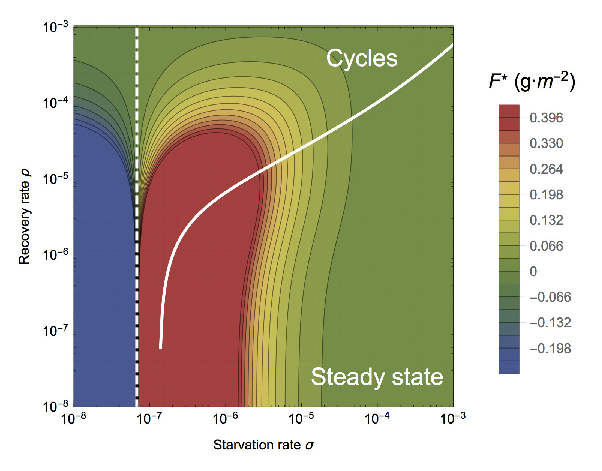
\includegraphics[width=0.45\textwidth]{fig_FixedPoint2.eps}
\caption{\small{ The transcritical (TC; dashed line) and Hopf bifurcation (solid line) as a
  function of the starvation rate $\sigma$ and recovery rate $\rho$ for a 100g consumer.  These
  bifurcation conditions separate parameter space into unphysical (left of the TC), cyclic,
  and steady state dynamic regimes.  The colors show the steady state densities for the energetically replete consumers $F^*$.  
  % Steady state densities for the energetically deficient consumers $H^*$ (not shown)
  % scale with those for $F^*$.  
}\label{fig:fp}}
\end{figure*}


\begin{figure*}[h!]
\centering
% 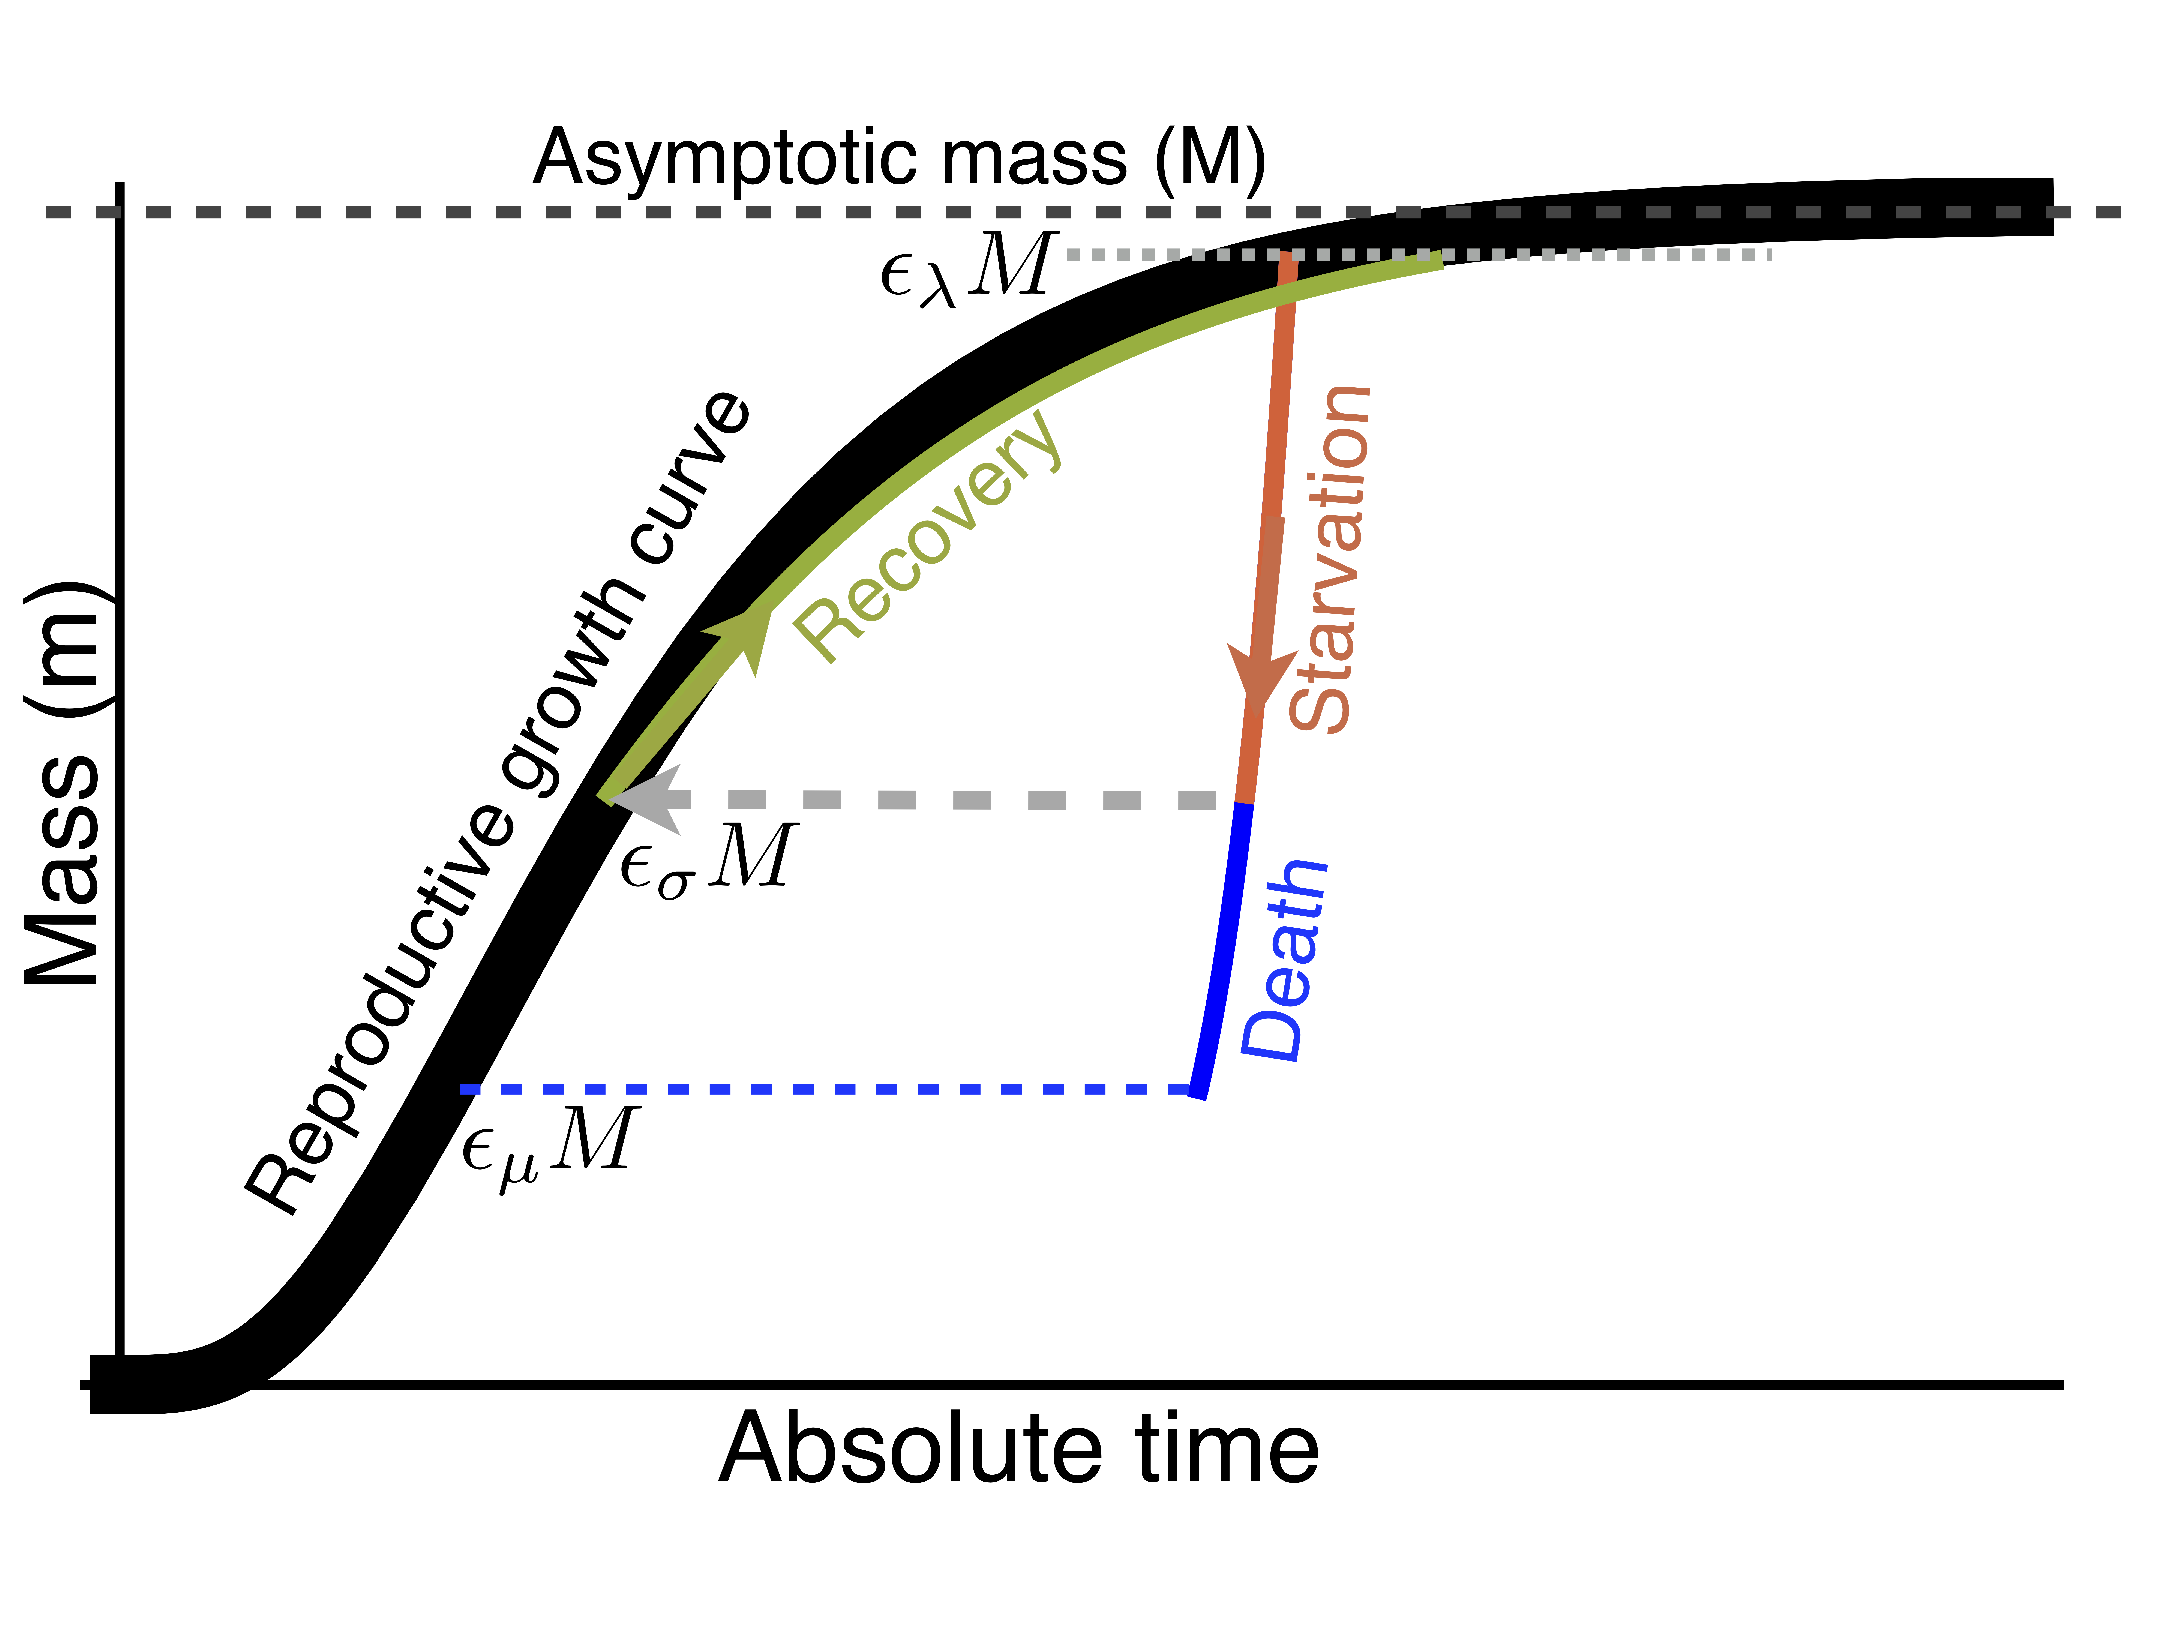
\includegraphics[width=0.4\textwidth]{Growth-trajectory-diagram.eps}
\caption{\small{ The growth trajectory over absolute time of an individual organism as a function of body mass.  
Initial growth follows the black trajectory to an energetically replete reproductive adult mass of $m=\epsilon_\lambda M$ (see Methods). %which we assume is 95\% asymptotic mass $M$.  
Starvation follows the red trajectory to $m = \epsilon_\sigma \epsilon_\lambda  M$. 
Recovery follows the green curve to the replete adult mass, where this trajectory differs from the original growth because only fat is being regrown which requires a longer time to reach $\epsilon_\lambda M$. %different energetics and 
Alternatively, death from starvation follows the blue trajectory to $m=\epsilon_\mu \epsilon_\lambda  M$.}\label{fig:growth}}
\end{figure*}


\begin{figure*}[h!]
\centering
% 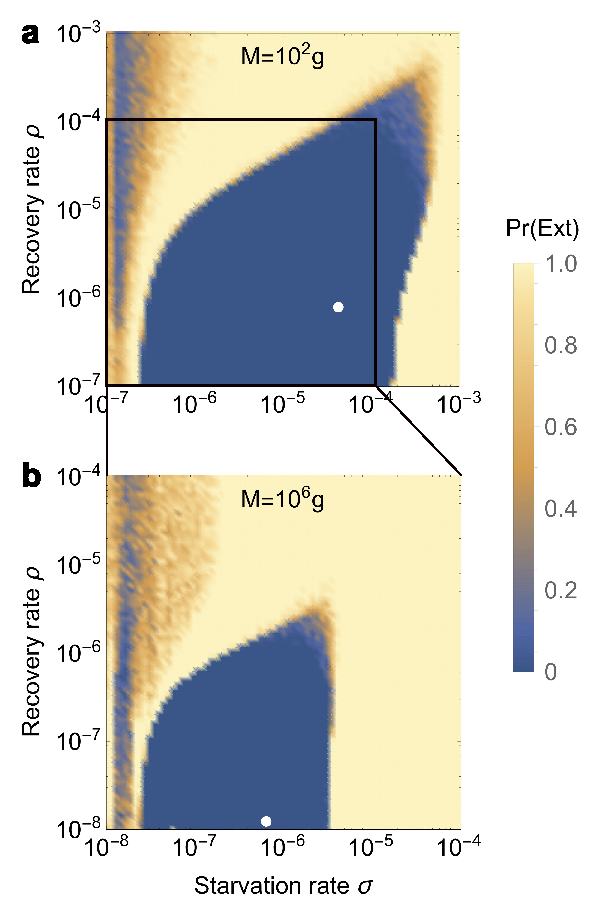
\includegraphics[width=0.4\textwidth]{fig_ExtinctionAllometricComb4.eps}
\caption{\small{ Probability of extinction for a consumer with ({\bf a}) $M=10^2$g and ({\bf b}) $M=10^6$g as a function of the starvation rate $\sigma$ and recovery rate $\rho$, where the initial density is given as $(XF^*,XH^*,R^*)$, where $X$ is a random uniform variable in $[0,2]$. Note the change in scale in panel {\bf b}.  Extinction is defined as the population trajectory falling below $0.2\times$ the allometrically constrained steady state. The white points denote the allometrically constrained starvation and recovery rate.}\label{fig:ext}}
\end{figure*}


\begin{figure*}[h!]
\centering
% 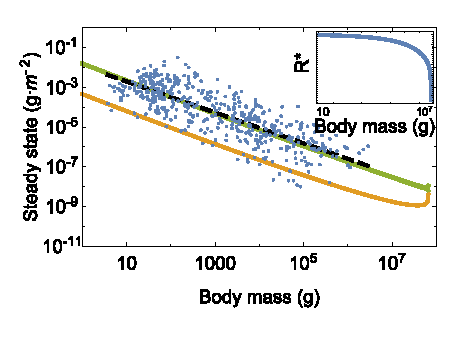
\includegraphics[width=0.4\textwidth]{fig_FPAllometric2.eps}
\caption{\small{Consumer steady states $F^*$ (green) and $H^*$ (orange) as a function of
  body mass along with the data from Damuth \citep{Damuth:1987kr}. Inset: Resource steady state $R^*$ as a function of consumer body mass.}\label{fig:mass}}
\end{figure*}


\begin{figure*}[h!]
\centering
% 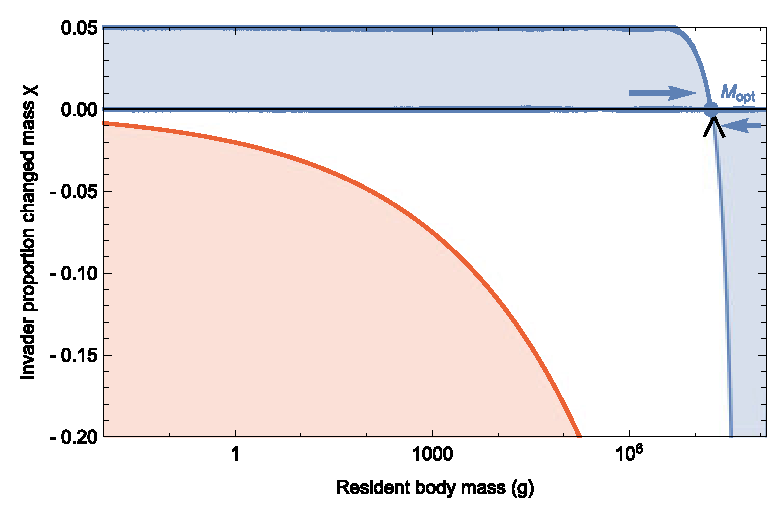
\includegraphics[width=0.4\textwidth]{fig_Invasion.eps}
\caption{\small{Competitive outcomes for a resident species with body mass
    $M$ vs. a closely related competing species with modified body mass
    $M^\prime=M(1+\chi)$.  The blue region denotes proportions of modified
    mass $\chi$ resulting in exclusion of the resident species.  The red
    region denotes values of $\chi$ that result in a mass that is below the
    starvation threshold and are thus infeasible.  Arrows point to the
    predicted optimal mass from our model $M_{\rm \rm opt}=1.748\times 10^7$,
    which may serve as an evolutionary attractor for body mass.  The black
    wedge points to the largest body mass known for terrestrial mammals
    (\emph{Deinotherium} spp.) at $1.74\times10^7$
    (g)~\citep{Smith:2010p3442}.}\label{fig:invasion}}
\end{figure*}



\end{document}
